\underline{\textbf{Вопросы при защите лабораторной работы}}\\
\begin{enumerate}
\item \textit{Приведите результаты тестирования программы (графики, общие соображения, качественный анализ)}

\begin{enumerate}
	\item $F_0(t) = 0$
	Из-за того, что тепловой поток равен нулю, температура равна $T_0$ для всех $x$.
	\begin{figure}[pt!]
	\begin{center}
		{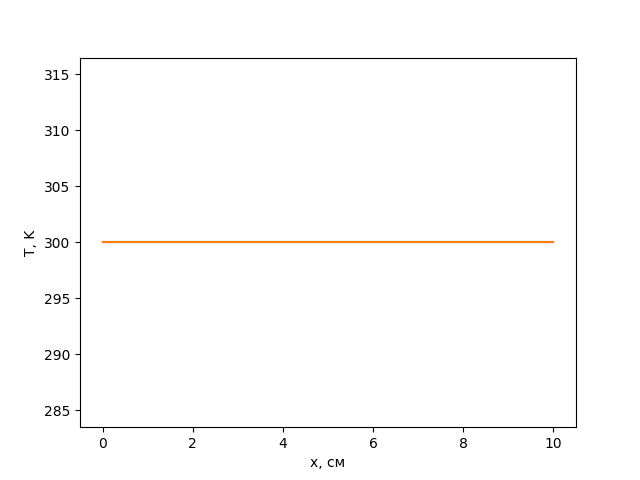
\includegraphics[height=6.5cm, width = 10cm]{../pictures/Figure_3}}
		\caption{Тест 1}
	\end{center}
	\end{figure}

\newpage

	\item $F_0(t) < 0$
	В такой ситуации происходит съём тепла.
	\begin{figure}[h]
		\begin{center}
			{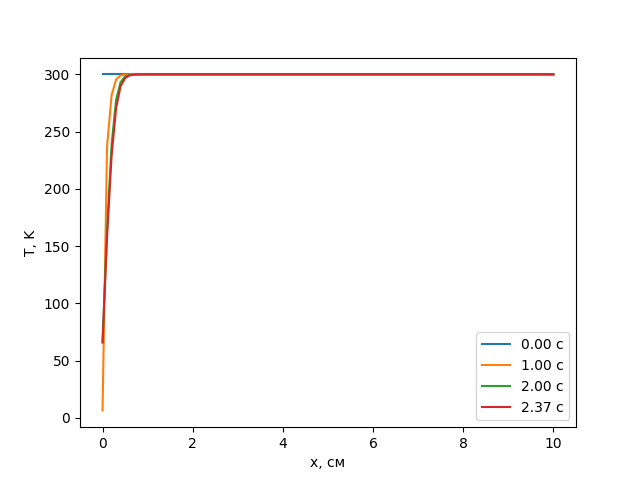
\includegraphics[height=6.5cm, width = 10cm]{../pictures/Figure_4}}
			\caption{Тест 2}
		\end{center}
	\end{figure}

	
\end{enumerate}
\end{enumerate}








